\begin{figure}[htb]
\centering
\caption{Causal Effects of Democracy}\label{fig:first-stage}
\captionsetup{width=0.8\textwidth}
\begin{subfigure}[c]{.49\linewidth}

    \centering
    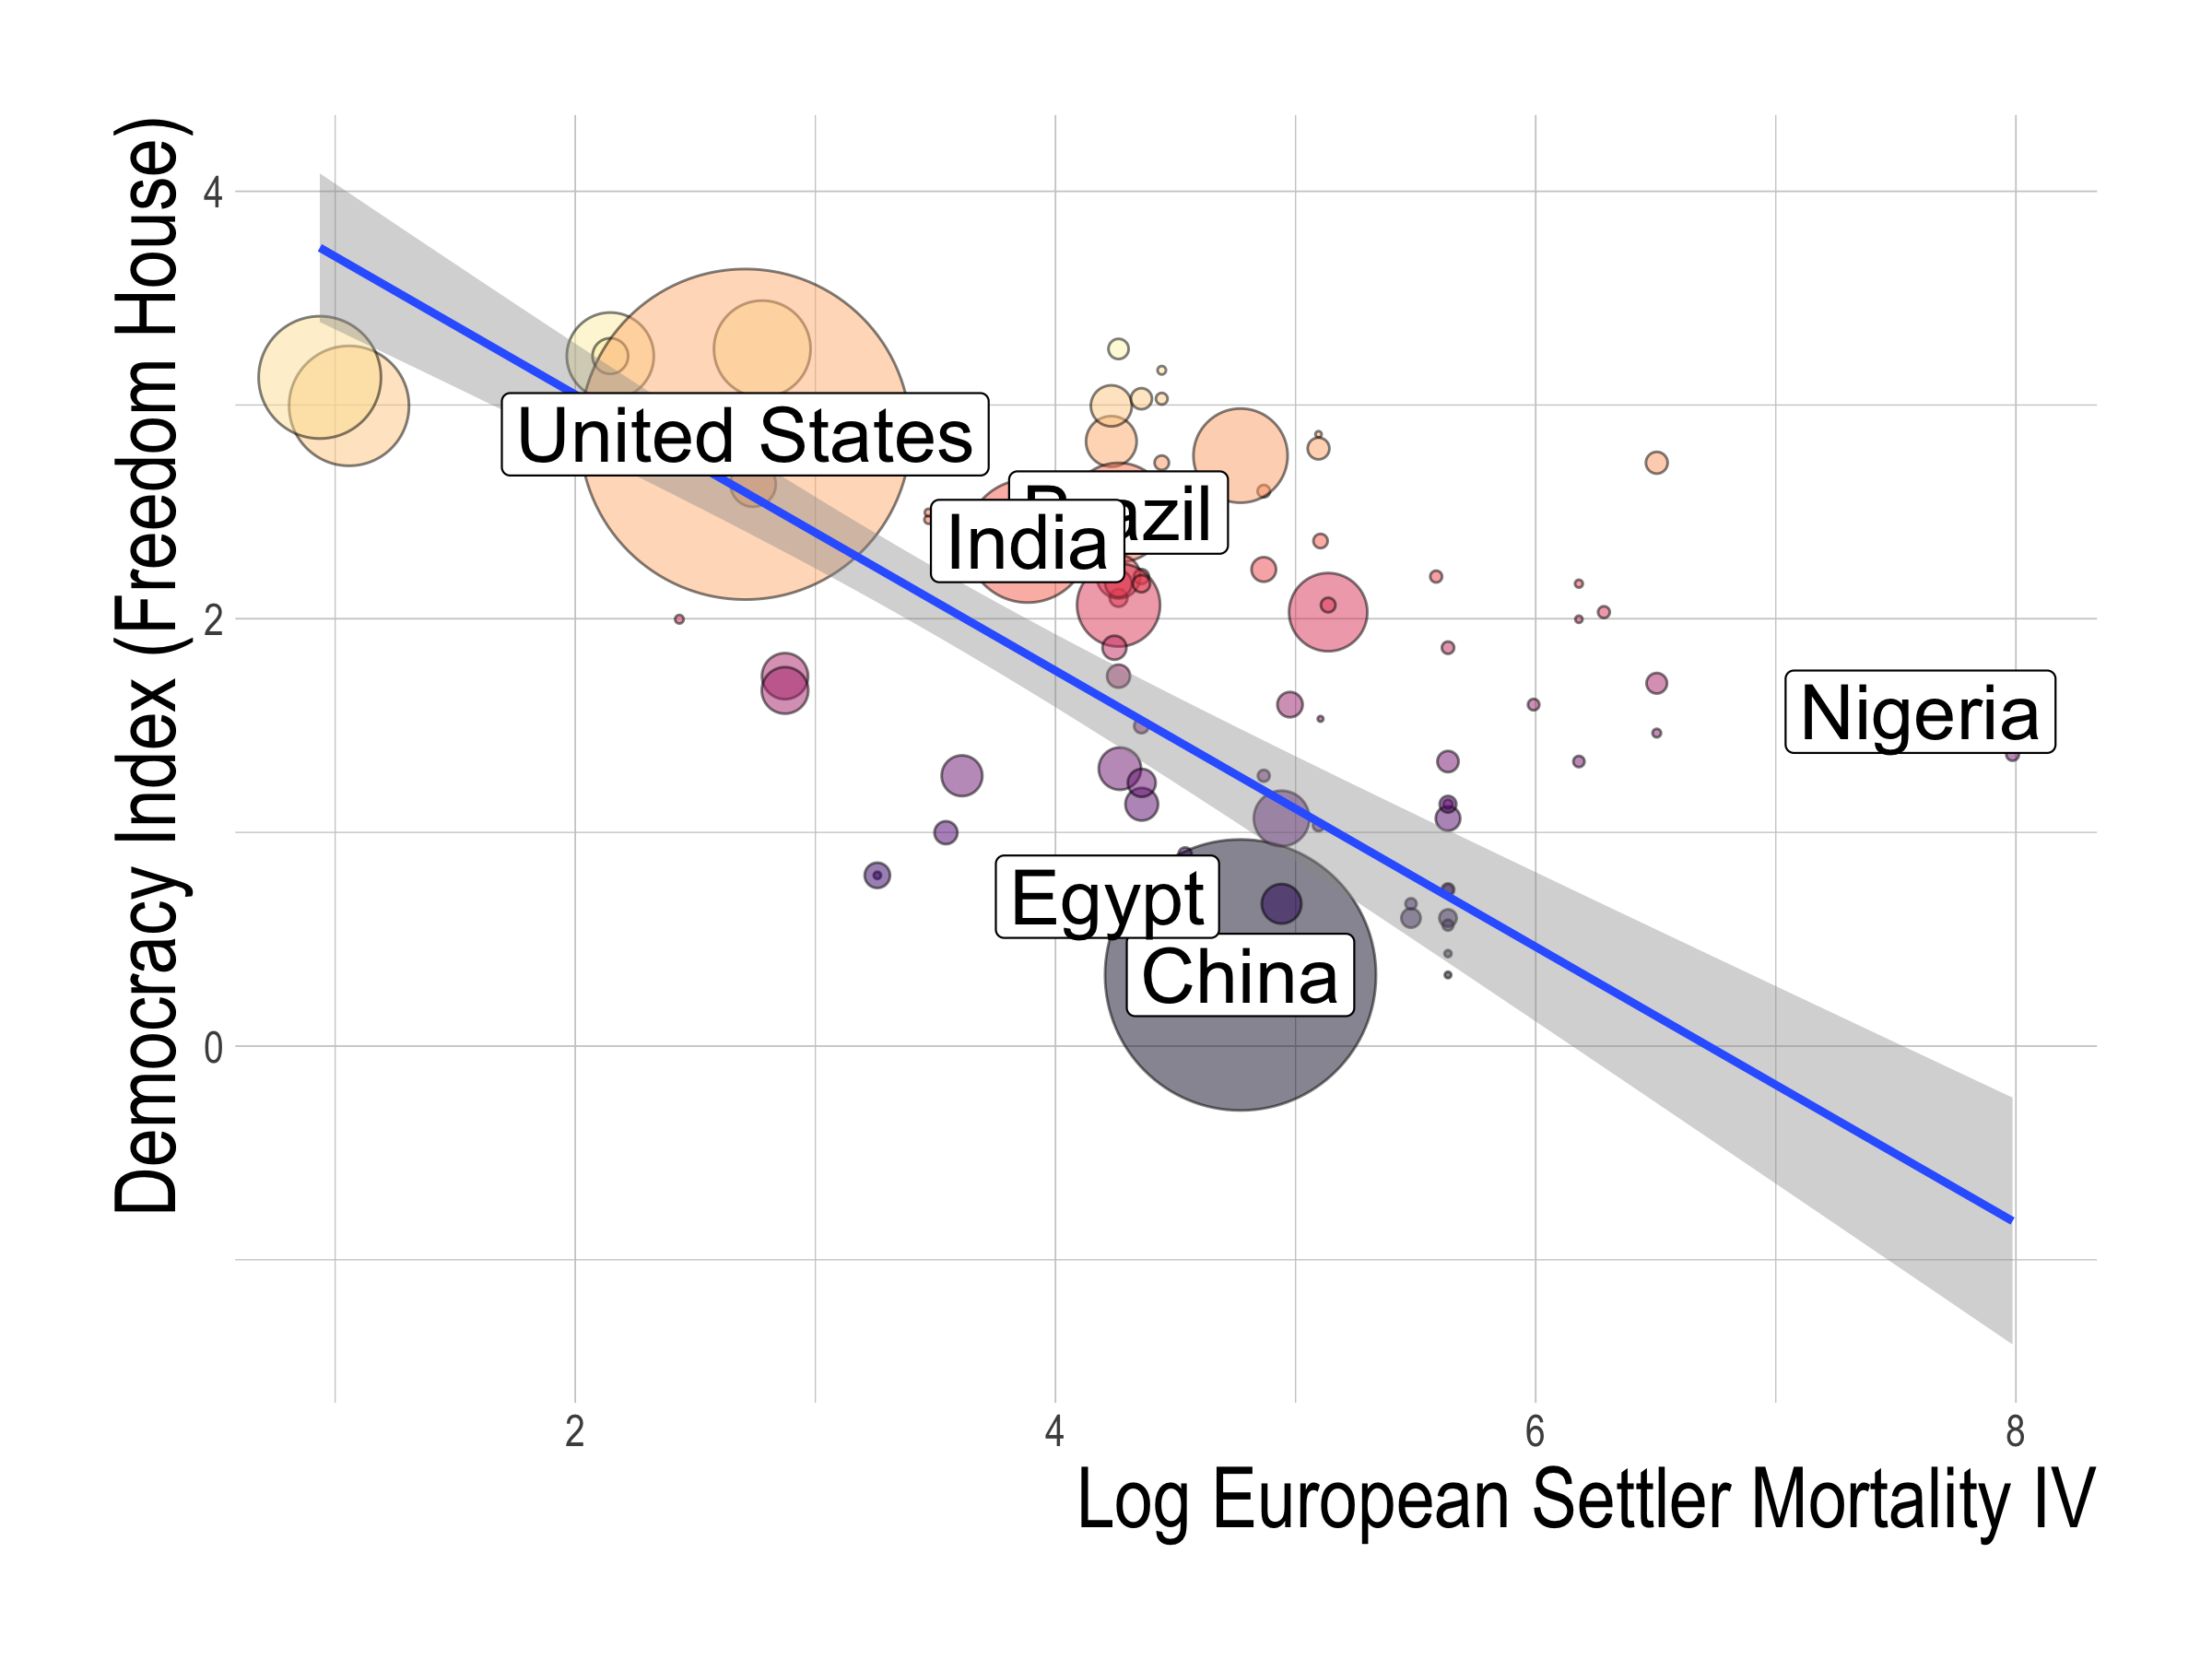
\includegraphics[width=.99\textwidth]{plots/figure2a.png}
    \caption{First-stage: Log European Settler Mortality IV}\label{fig:first-stage-european-settlers}
    
    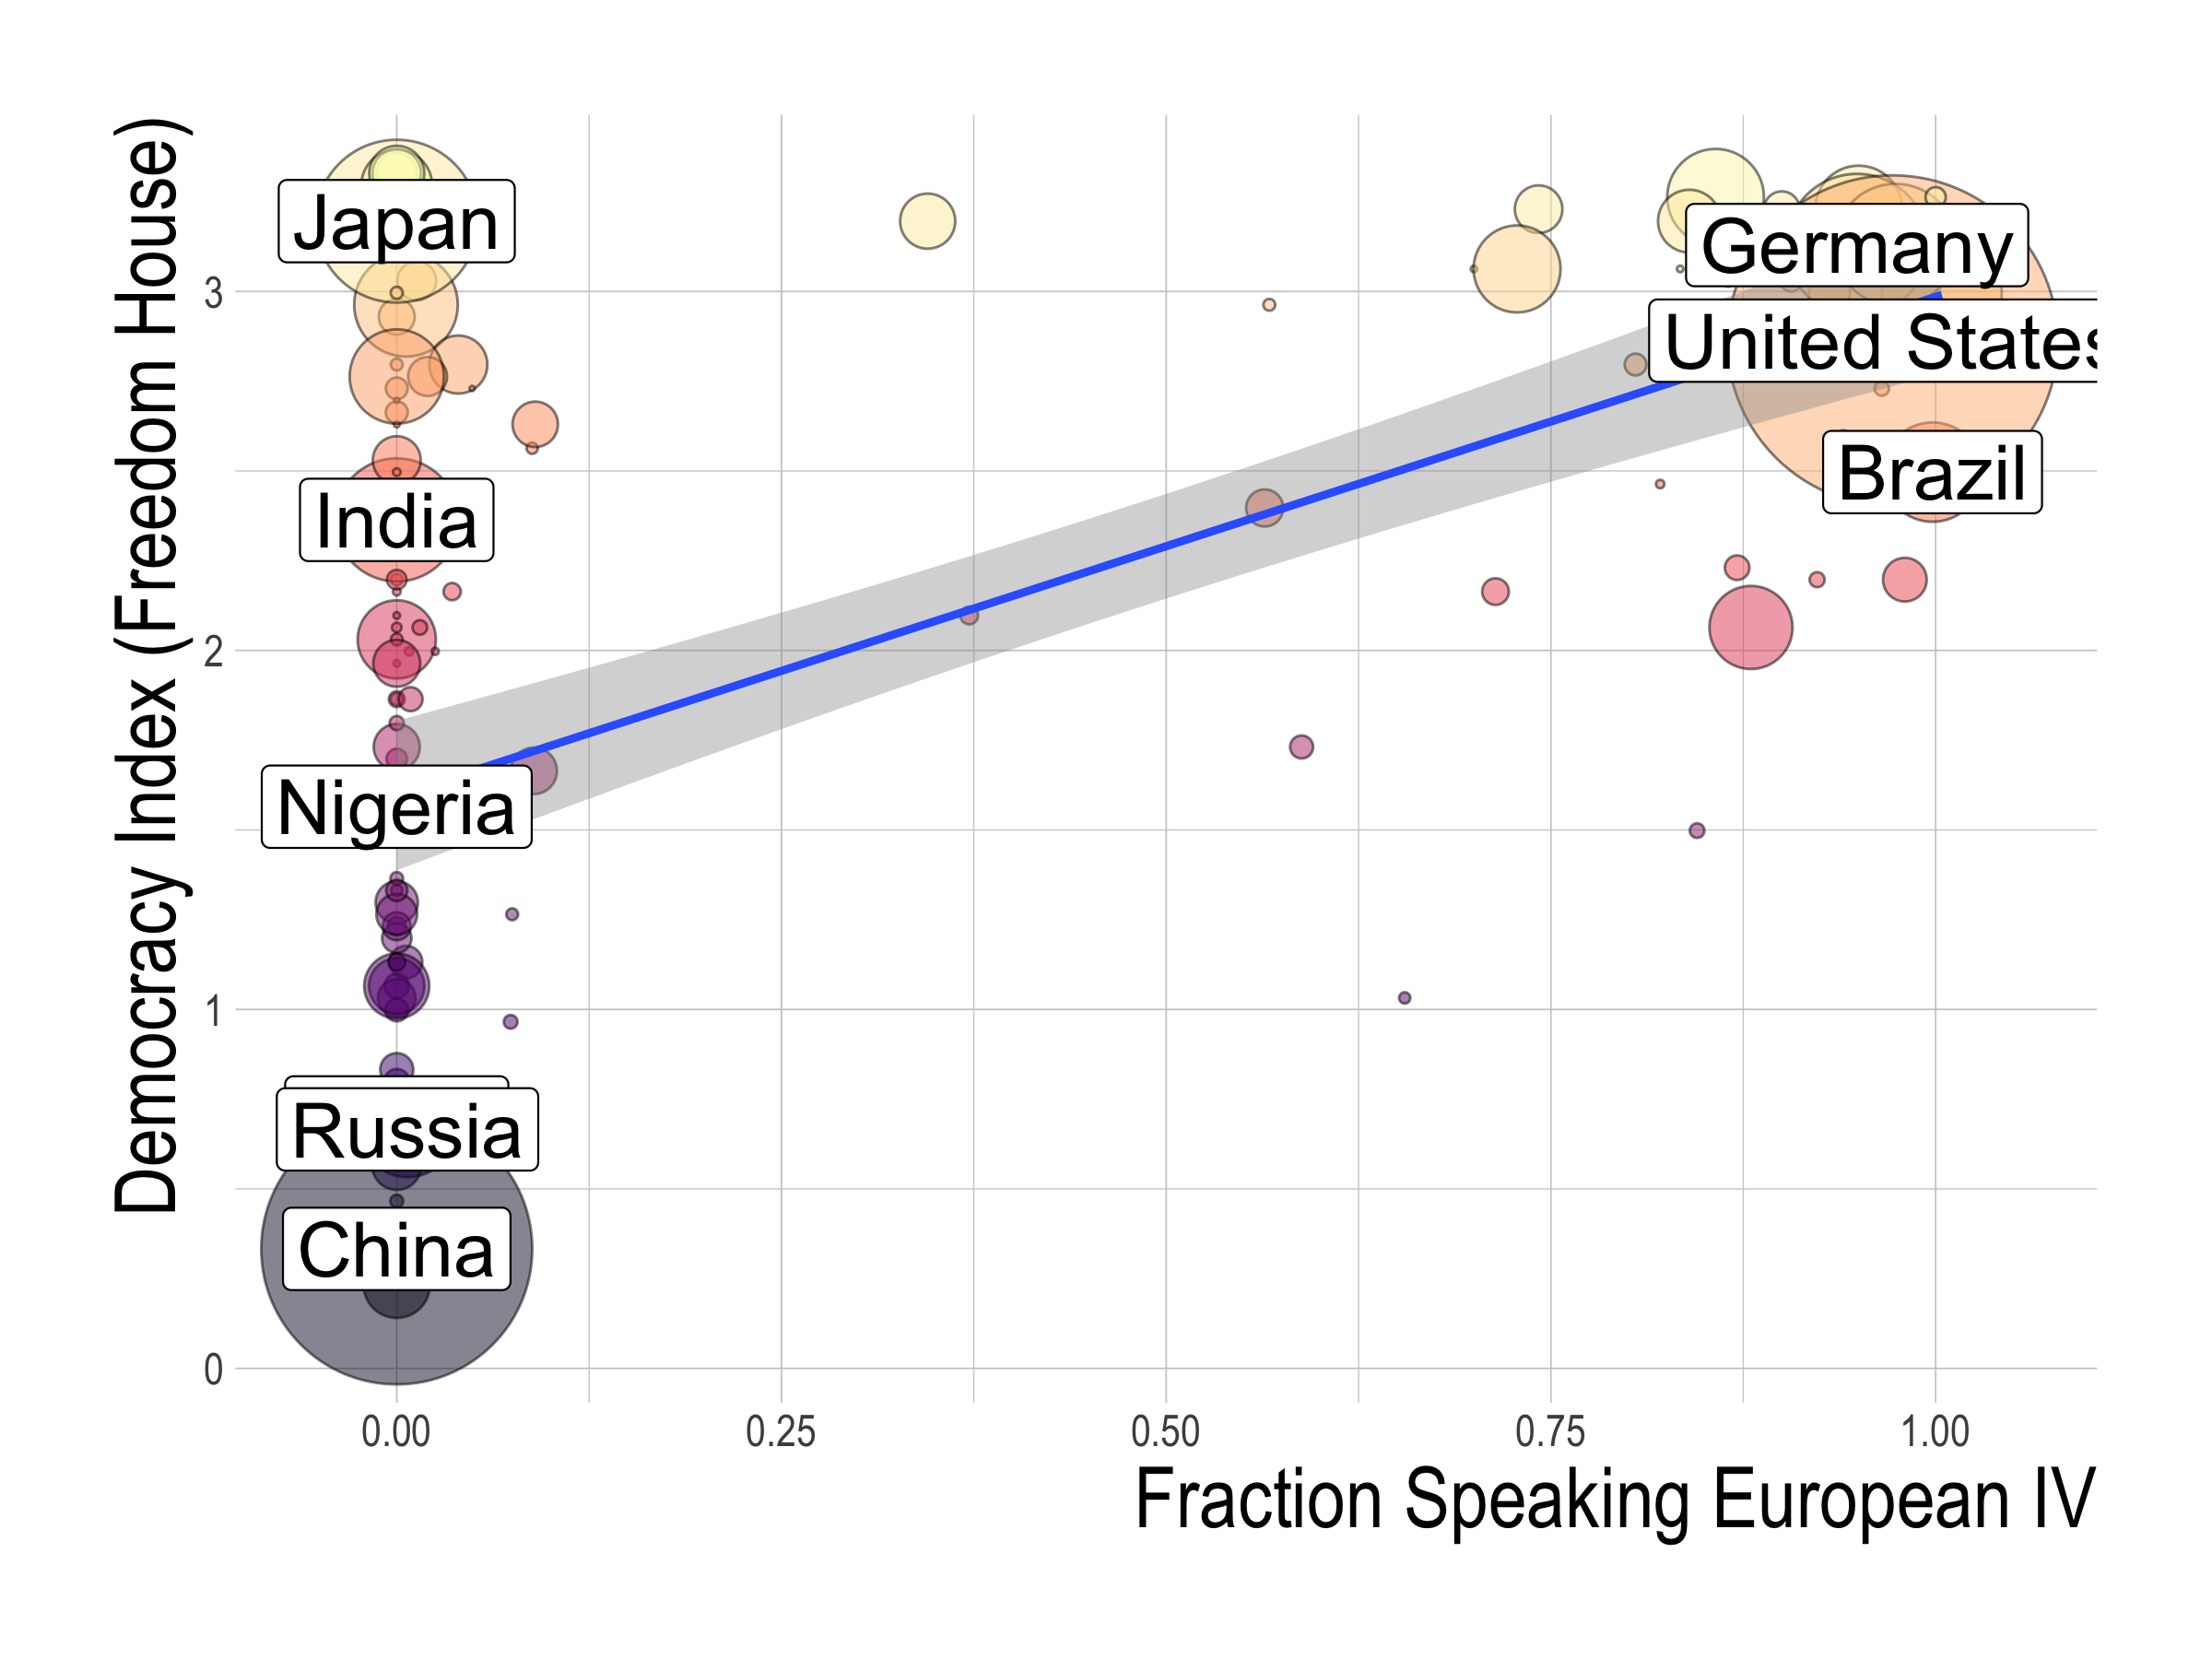
\includegraphics[width=.99\textwidth]{plots/figure2b.png}
    \caption{First-stage: Fraction Speaking European IV}\label{fig:first-stage-fraction-european}

\end{subfigure}
\begin{subfigure}[c]{.49\linewidth}
    \centering
    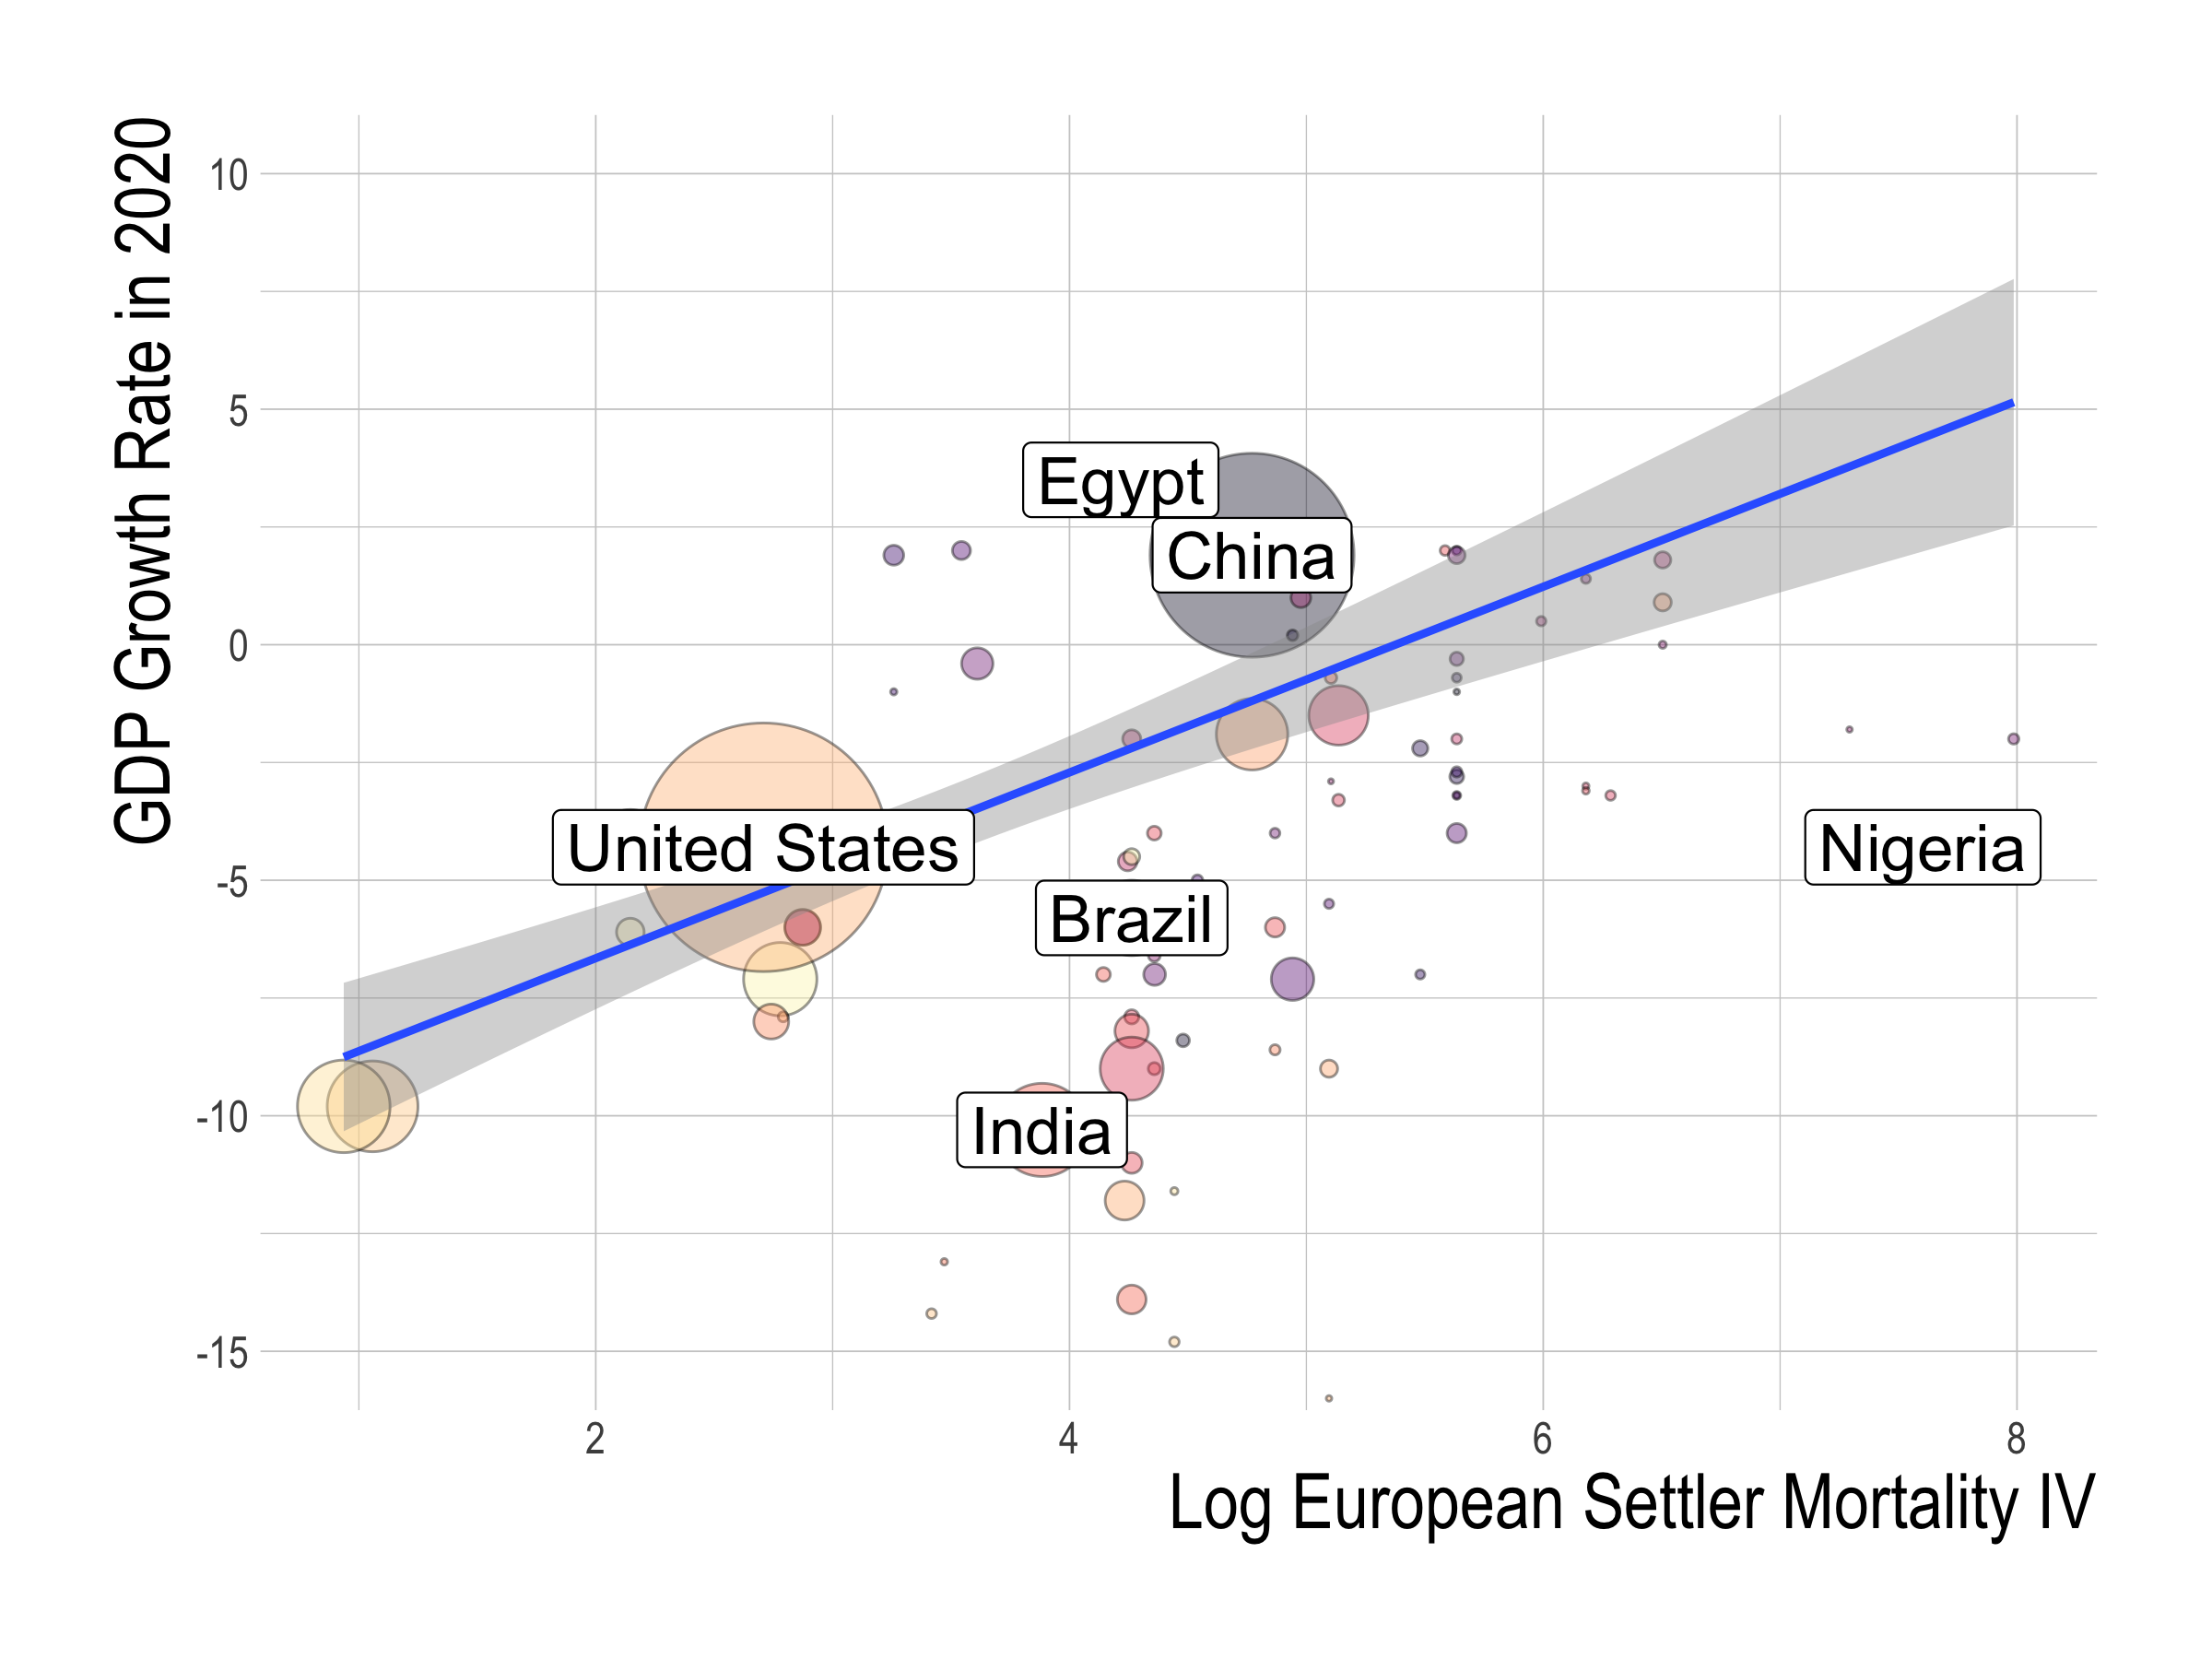
\includegraphics[width=.99\textwidth]{plots/figure2c.png}
    \caption{Reduced form: GDP Growth Rate in 2020}\label{fig:reduced-gdp-logem}
    
    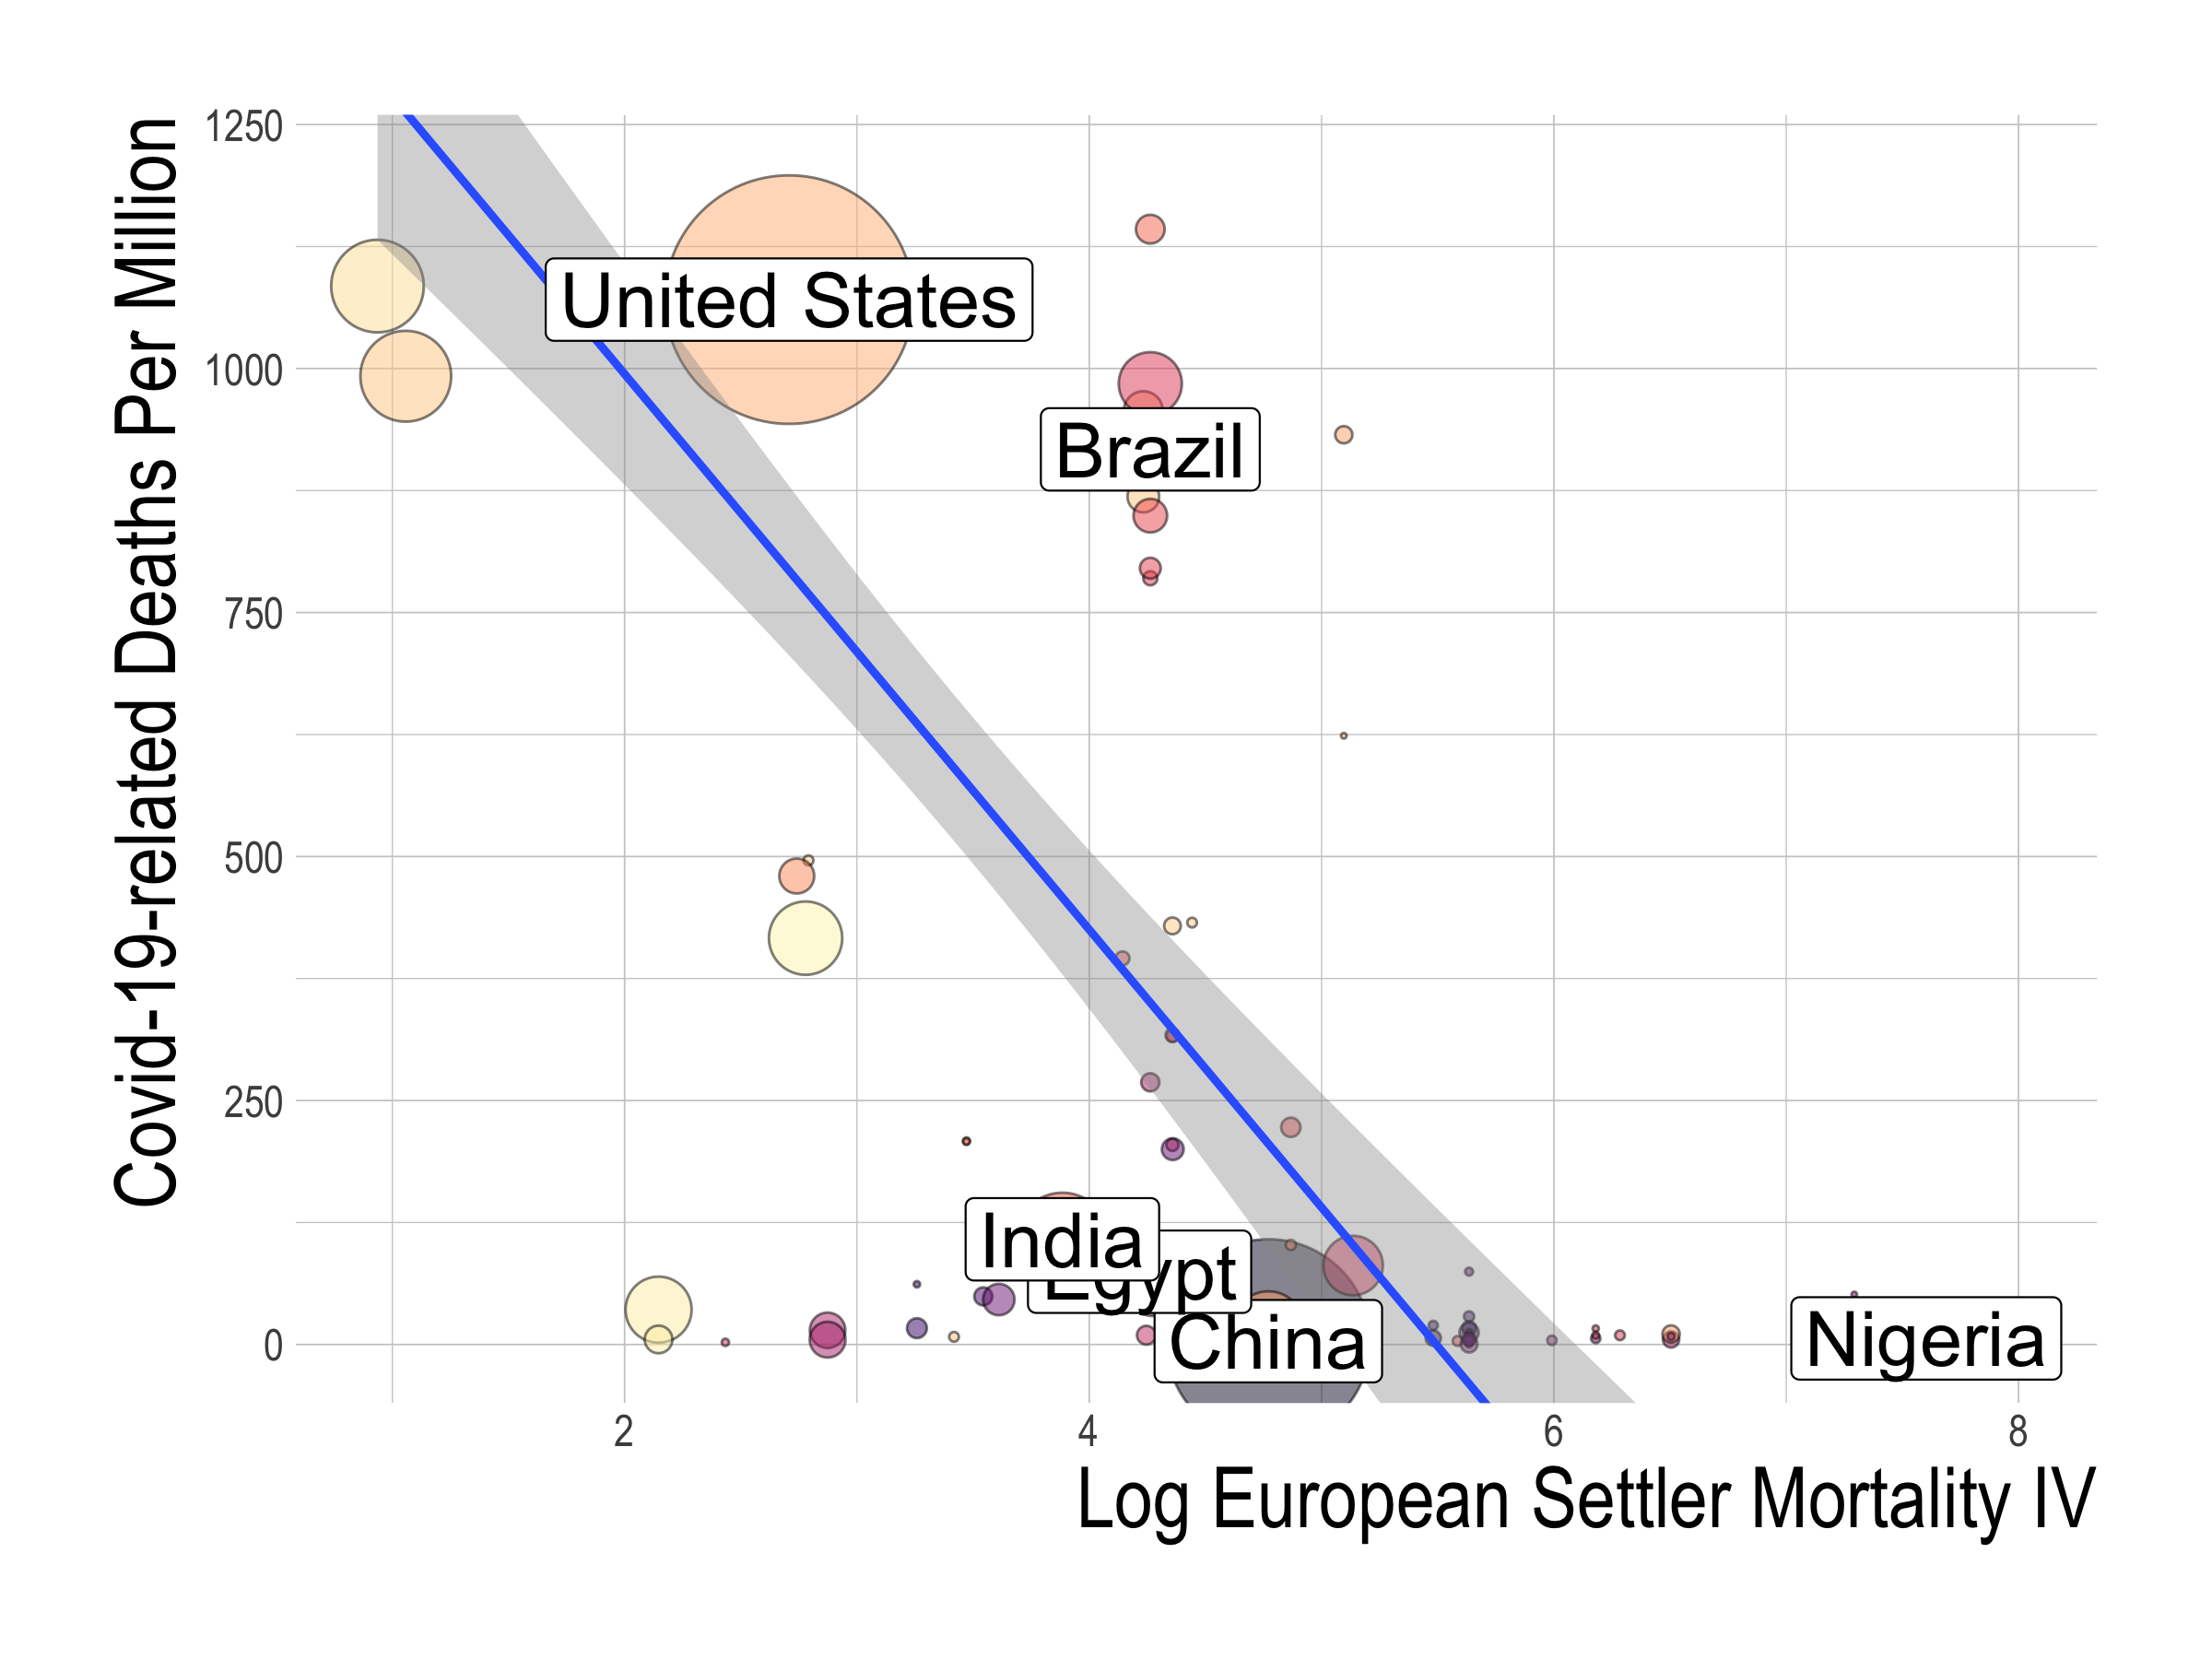
\includegraphics[width=.99\textwidth]{plots/figure2d.png}
    \caption{Reduced form: Covid-19-related Deaths Per Million}\label{fig:reduced-deaths-logem}
    
\end{subfigure}

\caption*{\textit{Notes:} Panels (a) and (b) show the first-stage relationship between democracy and two univariate IVs: the log European settler mortality IV and the fraction speaking European IV. Panels (c) and (d) show the reduced-form relationship between the log European settler mortality IV and Covid-19 outcomes: GDP growth rates in 2020 and Covid-19-related deaths per million. The Democracy Index (Freedom House) is the sum of the political rights and civil liberties scales from \emph{Freedom in the World 2020} by Freedom House. It is normalized to have standard deviation one. The size of each circle (country) is proportional to its GDP. The colors depend on the level of the democracy index. The line is the OLS regression fitted line without controls and weights countries by GDP. The shaded area corresponds to the 95\% confidence interval.}
\end{figure}

